\documentclass[10pt,a4paper]{article}
\usepackage[utf8]{inputenc}
\usepackage[T1]{fontenc}
\usepackage{amsmath}
\usepackage{amssymb}
\usepackage{graphicx}
\usepackage{hyperref}
\usepackage{csvsimple}
\usepackage{longtable}
\usepackage{array}
\usepackage{adjustbox}
\usepackage{float}
\usepackage{subcaption}
\usepackage{graphicx}
\usepackage{caption}

\title{Understanding Hidden Computations in Chain-of-Thought Reasoning}
\author{Aryasomayajula Ram Bharadwaj\\
Independent Researcher\\
\texttt{ram.bharadwaj.arya@gmail.com}}

\begin{document}

\maketitle

\begin{abstract}
Recent work has shown that transformer models can perform complex reasoning tasks using Chain-of-Thought (COT) prompting, even when the COT is replaced with filler characters. This paper attempts to investigates methods to decode these hidden/filler computations, focusing on the 3SUM task. We analyze a 34M parameter LLaMA model trained on filler COT sequences and propose a novel decoding method that successfully eliminates the filler tokens in the original COT without sacrificing the accuracy. Our findings provide insights into how transformers encode and process information in filler COT sequences, offering new perspectives on model interpretability and the nature of computation in language models.

\end{abstract}

\section{Introduction}
Chain-of-Thought (COT) prompting has emerged as a powerful technique for improving the performance of large language models on complex reasoning tasks [1]. However, recent work by [2] demonstrates that these improvements can be achieved even when the COT is replaced with hidden/filler characters (e.g., "..."), raising intriguing questions about the nature of computation being performed within these models.

This paper builds upon the findings of [2], focusing on the 3SUM task as a case study. We aim to decode the hidden computations embedded within the transformer architecture when trained on hidden COT sequences. Our work provides valuable insights into how these models encode and process information, potentially leading to improved model interpretability and more effective training strategies.

\section{Background}

\subsection{The 3SUM Task}
The 3SUM task involves finding three numbers in a given set that sum to zero. In this experiment it serves as a proxy for more complex reasoning tasks to study the computational capabilities of transformer models [1]. For this experiment we have used the same data representation method and generating process or 3SUM sequences as in [1].

\subsection{Chain-of-Thought using Filler Tokens}
In this variant of Chain-of-Thought, intermediate reasoning steps are replaced with filler characters (e.g., "..."). It has been observed in [1] that the models trained on hidden/filler sequences still perform well, suggesting that meaningful computation occurs despite the lack of explicit reasoning steps.

\section{Methodology}
We used a 34M-parameter LLaMA model with 4 layers, 384 hidden dimension, and 6 attention heads [4], the size of the training and test datasets and all other hyperparameters are kept the same as in the "Let's think dot by dot" paper [2]. Our analysis focused on three main areas: Layer-wise Representation Analysis, Token Ranking, and Modified Greedy Decoding Algorithm.

\section{Results and Discussion}

\subsection{Layer-wise Analysis}
Our analysis revealed a gradual evolution of representations across the model's layers. The initial layers primarily contained raw numerical sequences associated with the 3SUM problem's chain of thought. However, starting from the third layer, we noticed the emergence of hidden tokens. As we progressed through subsequent layers, we observed a steady transition from purely numerical sequences to an increasing prevalence of filler characters.
This pattern suggests that the model develops the ability to utilize filler tokens as proxies only in its deeper layers, which aligns with intuitive expectations of how neural networks process information. After conducting a comprehensive evaluation across numerous examples, we found that, on average, there is a marked increase in filler token usage immediately following the second layer. Furthermore, the final layers of the model demonstrate extensive reliance on these hidden tokens.
For this analysis, we employed nostalgebraist's logit lens method [3].

\begin{figure}[H]
\centering

\includegraphics[width=\textwidth]{hidden_tokens_percentage_by_layer.png}
\caption{Filler token occurrence percentages in generated sequences across layers}
\label{fig:hidden_token_percentages}
\end{figure}


\subsection{Token Rank Analysis}
The top-ranked token was consistently the filler character ("."), while lower-ranked tokens revealed the original, non-filler COT sequences. This supports the hypothesis that the model replaces all computation with filler tokens on top while keeping the original computation intact underneath. We have provided a sample snapshot of sequences decoded at each layer for both the top (rank-1) and rank-2 tokens in the appendix section.

\subsection{Modified Greedy Decoding Algorithm}
Based on the observations made in the token rank analysis, We implemented a modified greedy autoregressive decoding method. The steps include: performing standard greedy decoding, selecting the second-highest probability token when encountering a filler token, and continuing this process for the entire sequence. This resulted in a 100\% match in 3SUM task results with and without filler tokens. To test the effectiveness of this method, we have also compared this with replacing the filler token with randomly sampled token instead of the next highest (rank-2) token. The percentages of the original and these modified decoding methods are visualized as plots below. 

\begin{figure}[H]
\centering
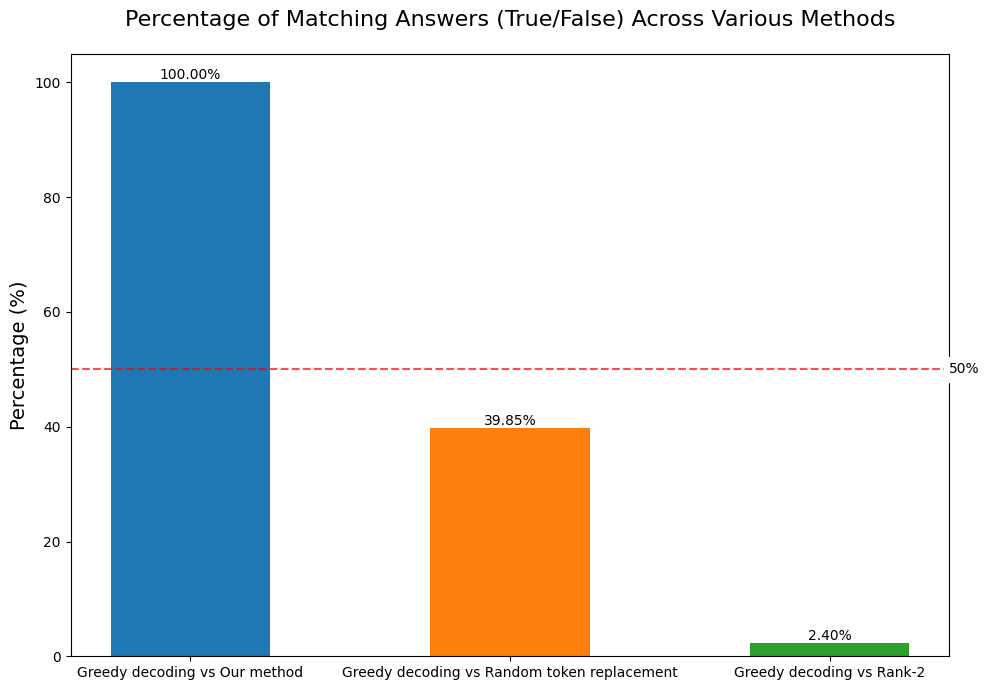
\includegraphics[width=\textwidth]{token_comparison_percentages.png}
\caption{Comparison of decoding methods}
\label{fig:decoding_comparison}
\end{figure}

\section{Implications and Future Work}
Our findings provide new tools for understanding internal reasoning processes and increase confidence in COT-based approaches for improving visibility. Future work should focus on developing better decoding methods or finding circuits that hide tokens, investigating generalizability to tasks beyond 3SUM (including natural language tasks), and improving token hiding methods (currently limited to one filler token which is simple to decode).

\clearpage
\section{Conclusion}
We have presented a novel approach to understanding hidden computations in transformer models through the analysis of token rankings and layer-wise representations, and the development of a modified decoding algorithm. Our insights into how models encode and process information in filler COT sequences open new avenues for improving interpretability, efficiency, and safety in language models. This work strengthens the belief in COT visibility research for interpretability.
\vfill
The code used for the experiments and analysis in this paper is available on GitHub at \href{https://github.com/rokosbasilisk/filler_tokens/tree/v2}{https://github.com/rokosbasilisk/filler\_tokens/tree/v2}.
\clearpage
\begin{figure}[p]
    \centering
    \section{Appendix: Layerwise view of sequences generated via various decoding methods}
    \vspace{-0.5em}  % Reduce space after the title
    
    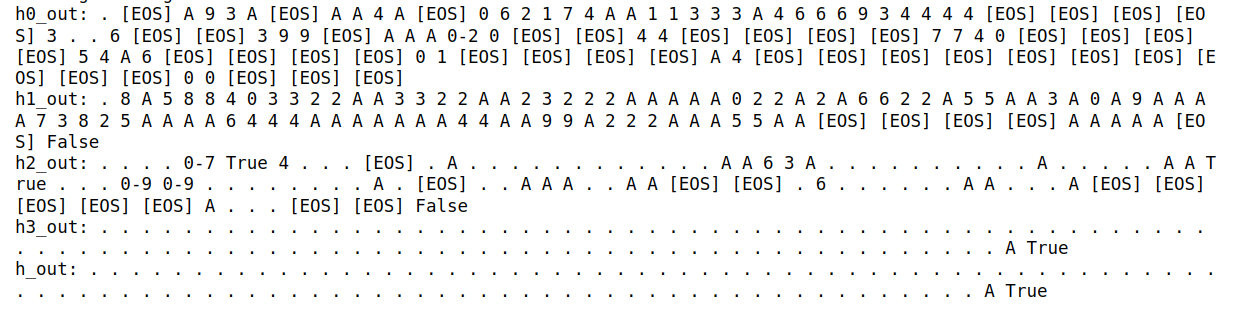
\includegraphics[width=\textwidth,height=0.19\textheight,keepaspectratio]{greedy_decoding.png}
    \captionof{figure}{Greedy Decoding}
    \label{fig:greedy}
    
    \vspace{0.5em}
    
    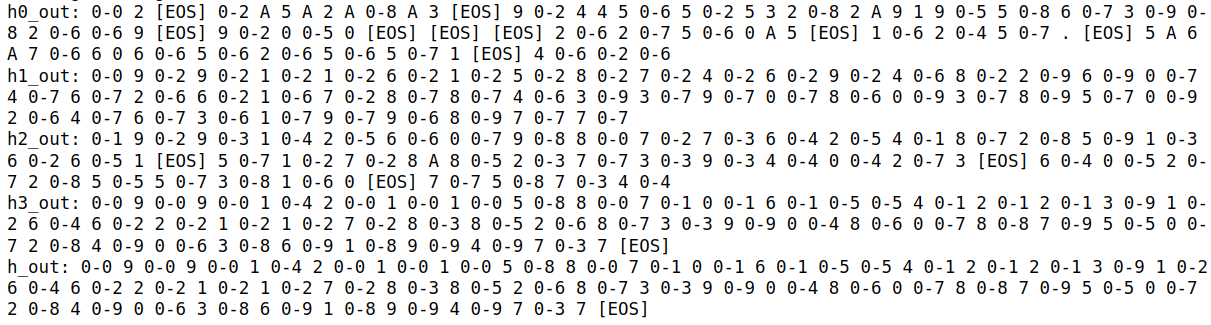
\includegraphics[width=\textwidth,height=0.19\textheight,keepaspectratio]{rank2_decoding.png}
    \captionof{figure}{Greedy Decoding with Rank-2 Tokens}
    \label{fig:rank2}
    
    \vspace{0.5em}
    
    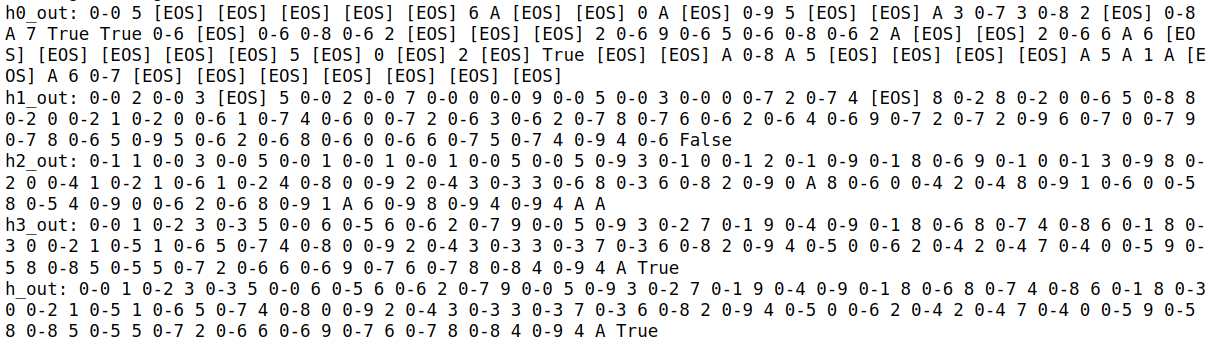
\includegraphics[width=\textwidth,height=0.19\textheight,keepaspectratio]{our_method_decoding.png}
    \captionof{figure}{Our Method: Greedy Decoding with Filler Tokens Replaced by Rank-2 Tokens}
    \label{fig:our-method}
    
    \vspace{0.5em}
    
    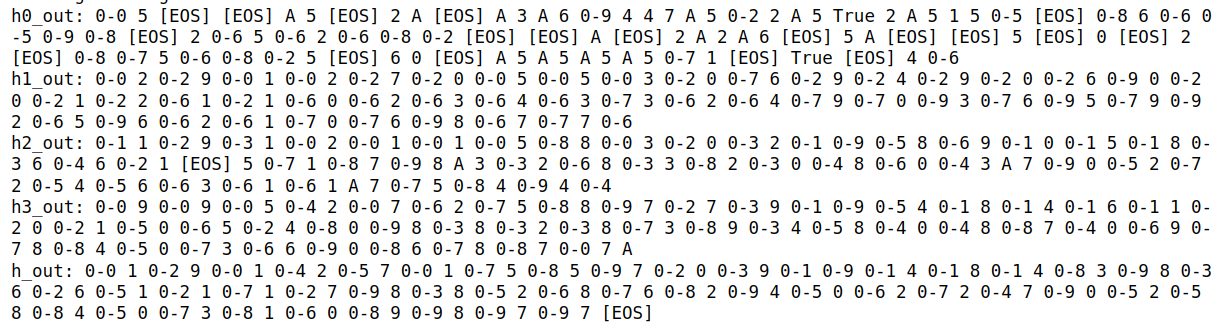
\includegraphics[width=\textwidth,height=0.19\textheight,keepaspectratio]{random_tokens_decoding.png}
    \captionof{figure}{Greedy Decoding with Filler Tokens Replaced by Randomly Selected Tokens}
    \label{fig:random}
\end{figure}

\clearpage

\begin{thebibliography}{9}

\bibitem{pfau2024let}
Pfau, J., Merrill, W., \& Bowman, S. R. (2023). Let's Think Dot by Dot: Hidden Computation in Transformer Language Models. \href{https://arxiv.org/abs/2404.15758}{arXiv:2404.15758}.

\bibitem{wei2022chain}
Wei, J., Wang, X., Schuurmans, D., Bosma, M., Ichter, B., Xia, F., ... \& Zhou, D. (2022). Chain-of-thought prompting elicits reasoning in large language models. \href{https://arxiv.org/abs/2201.11903}{arXiv:2201.11903}.

\bibitem{nostalgebraist2020}
nostalgebraist (2020). interpreting GPT: the logit lens \href{https://www.lesswrong.com/posts/AcKRB8wDpdaN6v6ru/}{interpreting-gpt-the-logit-lens}

\bibitem{touvron2023llama}
Touvron, H., Lavril, T., Izacard, G., Martinet, X., Lachaux, M. A., Lacroix, T., ... \& Lample, G. (2023). LLaMA: Open and Efficient Foundation Language Models. \href{https://arxiv.org/abs/2302.13971}{arXiv:2302.13971}.

\end{thebibliography}

\end{document}
